
\begin{figure}[h]
    \centering
    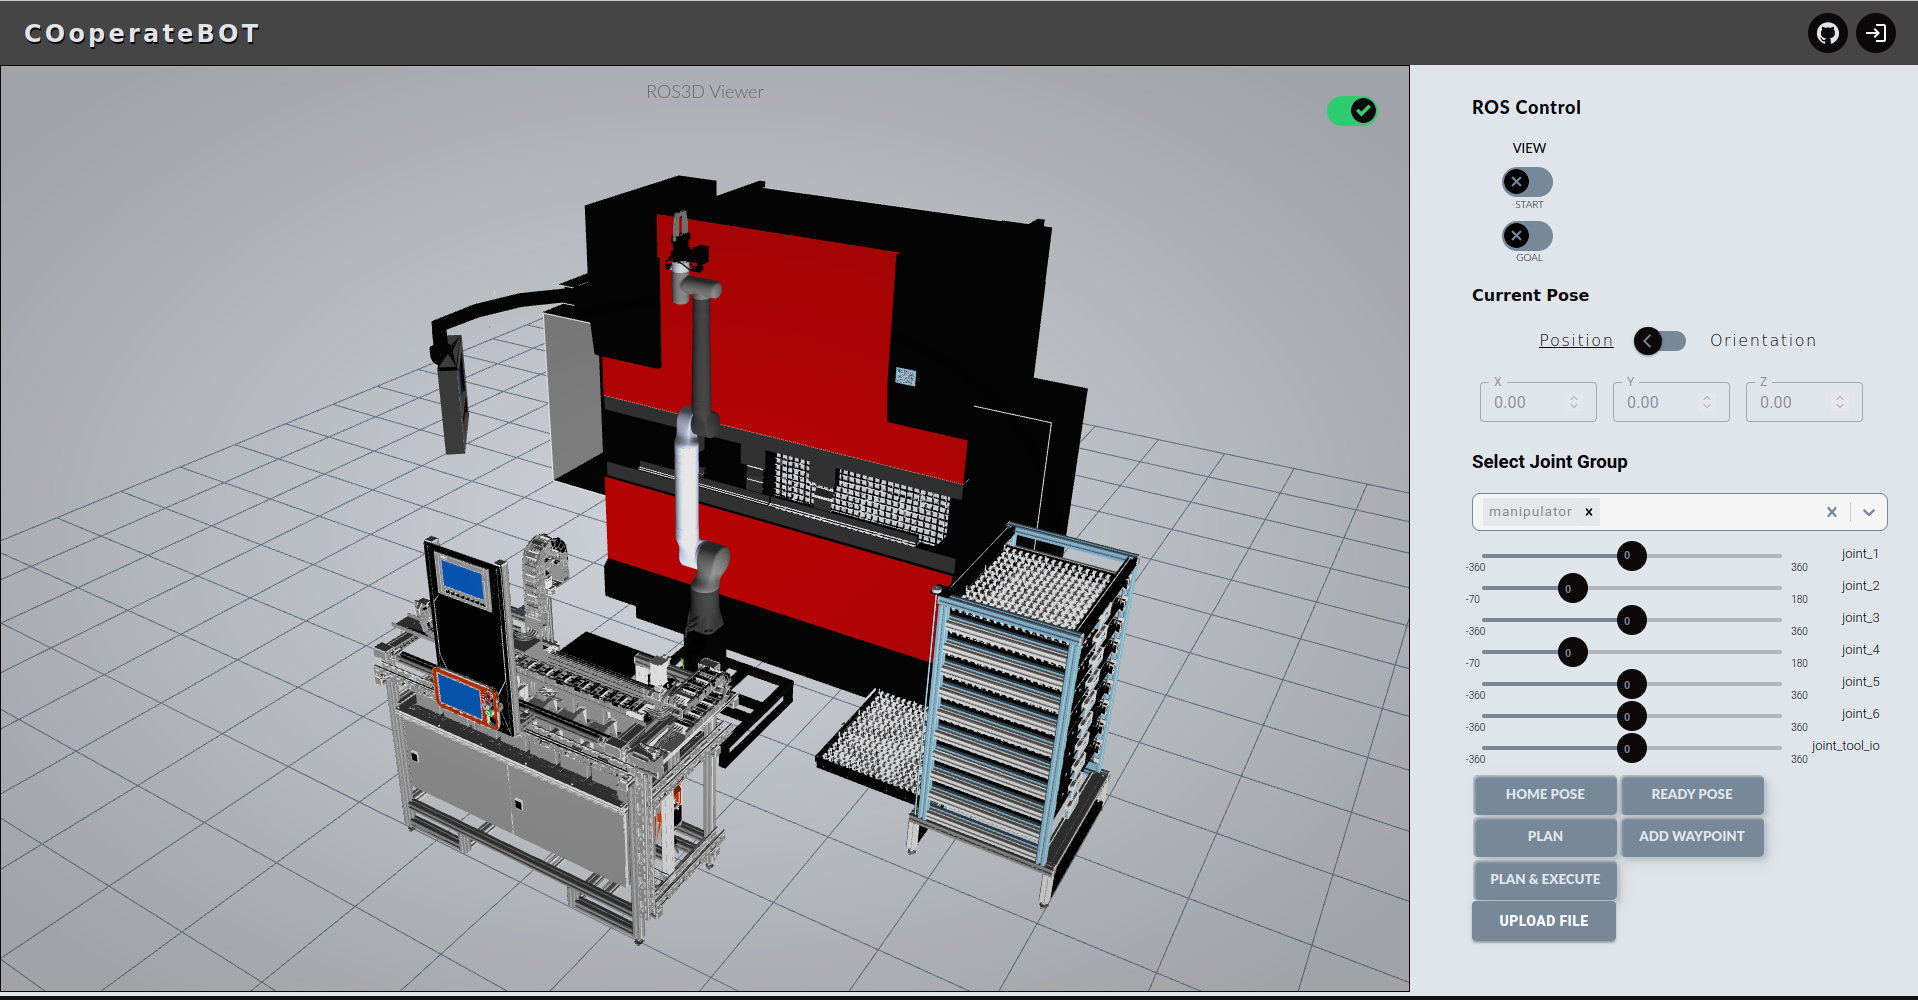
\includegraphics[width=1\textwidth]{figures/webui/webui0.png}
    \caption{Web User Interface}
    \label{fig:web-ui}
\end{figure}

\subsection{Viewer}
\label{subsec:web-ui-viewer}
The Viewer component provides a 3D visualization of the robot model within the web application. It leverages ros3djs to render a real-time representation of the robot, including its physical structure, sensor data, and environment. Users can manipulate the camera to explore the robot from various angles, zoom in and out, and observe its movements in real-time as it receives ROS data.

The viewer is customizable, with options to control the size, background color, and field of view to optimize visualization based on user needs. This is particularly useful for monitoring the robot's operations in complex environments, such as simulations or real-world tasks.


\subsection{Auto connection}
\label{subsec:web-ui-auto-connection}


\subsection{Robot URDF Visualization}
\label{subsec:web-ui-urdf-visualization}

\subsection{Interactive Marker}
\label{subsec:web-ui-interactive-marker}


\subsection{ROS Control Panel}
\label{subsec:web-ui-ros-control}
Simulation Mode, Robot mode


\begin{figure}[h]
    \centering
    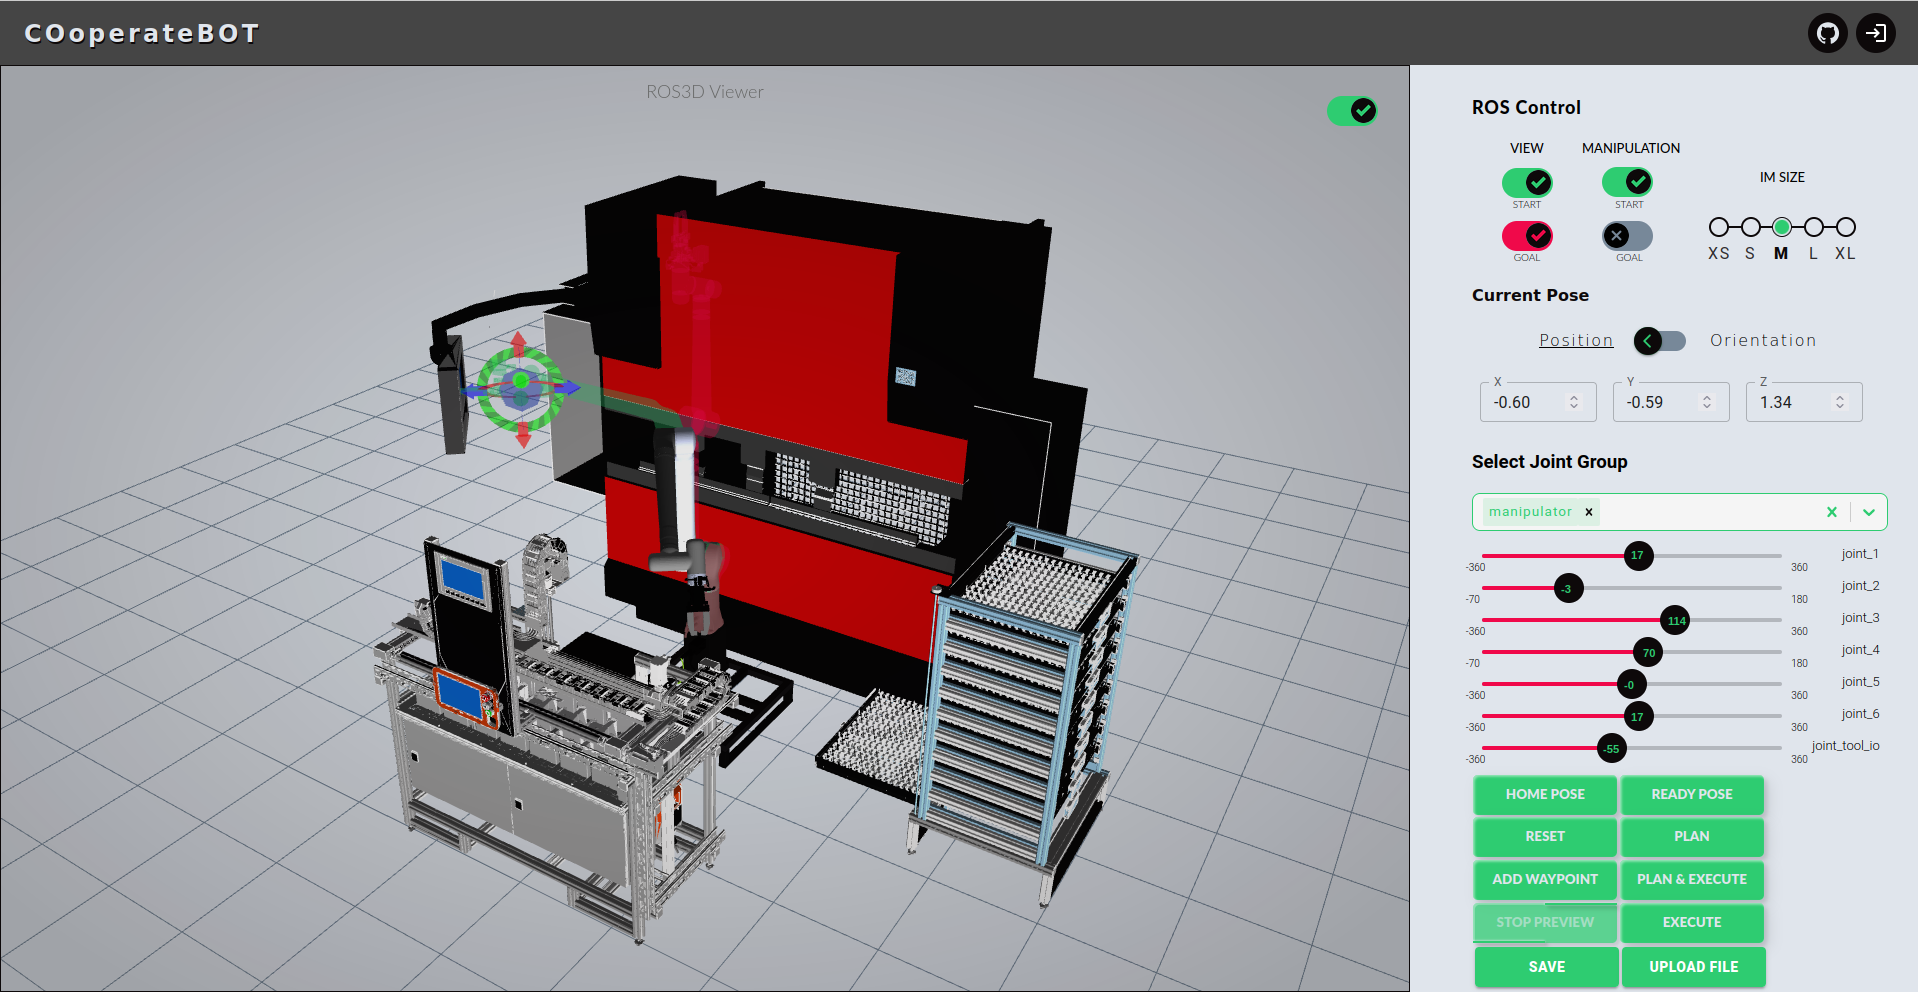
\includegraphics[width=1\textwidth]{figures/webui/web-ui-preview.png}
    \caption{Web User Interface previewing task execution}
    \label{fig:web-ui-preview}
\end{figure}

\subsubsection{Joint Slider}
\label{subsubsec:web-ui-joint-slider}

\subsubsection{Current Pose}
\label{subsubsec:web-ui-current-pose}

\subsubsection{View and Manipulation}
\label{subsubsec:web-ui-view-manipulation}

\subsubsection{IM Size}
\label{subsubsec:web-ui-im-size}


\subsubsection{Buttons}
\label{subsubsec:web-ui-buttons}

\subsection{Saving and loading path}
\label{subsec:web-ui-saving-path}

